\documentclass[a4paper,10pt]{report}
\usepackage{cours}
\usepackage{tkz-tab}

\begin{document}
\everymath{\displaystyle}

\begin{center}
 \shadowbox{{\huge TD 1 : Rappels d'analyse}}
\end{center}

\bigskip

%\maketitle{TD 1}{Rappels d'analyse}

\setlength{\shadowsize}{2pt} 


%\begin{center}
%{\large \textit{\underline{Convergence de suites}}}
%\end{center}
%%\begin{center}
%{\large \textbf{Exercices d'applications}}
%\end{center}

\begin{Exa}[Convergence de suites]
On pose pour tout $n \in \mathbb{N}^*$, 
    \[
    u_n = \sum_{k = 1}^n {\frac{1}{\sqrt k}} - 2\sqrt n \; \hbox{ et } \; v_n = \sum_{k = 1}^n {\frac{1}{\sqrt k}} - 2\sqrt {n + 1}
    \]
 Montrer que les suites $(u_n)_{n \geq 1}$ et $(v_n)_{n \geq 1}$ sont convergentes.
 \end{Exa}
 
 
\corr Montrons que $(u_n)_{n \geq 1}$ et $(v_n)_{n \geq 1}$ sont adjacentes.

\begin{itemize}
\item Soit $n \in \mathbb{N}^*$. Alors :
\begin{align*}
u_{n+1}-u_n & =  \sum_{k = 1}^{n+1} {\frac{1}{\sqrt k}} - 2\sqrt{n+1}  -\sum_{k = 1}^n {\frac{1}{\sqrt k}} + 2\sqrt{n}  \\
& = \dfrac{1}{\sqrt{n+1}} - 2 (\sqrt{n+1}-\sqrt{n}) \\
& = \dfrac{1}{\sqrt{n+1}} - 2 \times \dfrac{n+1-n}{\sqrt{n+1}+ \sqrt{n}} \\
& = \dfrac{1}{\sqrt{n+1}} - \dfrac{2}{\sqrt{n+1}+ \sqrt{n}}
\end{align*}
Pour tout entier $n \geq 1$,
$$ 0< \sqrt{n+1} + \sqrt{n} \leq 2 \sqrt{n+1}$$
donc par décroissance de la fonction inverse sur $\mathbb{R}_+^{*}$ :
$$ \dfrac{1}{\sqrt{n+1}+ \sqrt{n}} \geq \dfrac{1}{2 \sqrt{n+1}}$$
ou encore :
$$ \dfrac{2}{\sqrt{n+1}+\sqrt{n}} \geq \dfrac{1}{\sqrt{n+1}}$$
et ainsi :
$$ u_{n+1}-u_n \leq 0$$
La suite $(u_n)_{n \geq 1}$ est donc décroissante.
\item Soit $n \in \mathbb{N}^*$. Alors :
\begin{align*}
v_{n+1}-v_n & =  \sum_{k = 1}^{n+1} {\frac{1}{\sqrt k}} - 2\sqrt{n+2}  -\sum_{k = 1}^n {\frac{1}{\sqrt k}} + 2\sqrt{n+1}  \\
& = \dfrac{1}{\sqrt{n+1}} - 2 (\sqrt{n+2}-\sqrt{n+1}) \\
& = \dfrac{1}{\sqrt{n+1}} - 2 \times \dfrac{n+2-(n+1)}{\sqrt{n+2}+ \sqrt{n+1}} \\
& = \dfrac{1}{\sqrt{n+1}} - \dfrac{2}{\sqrt{n+2}+ \sqrt{n+1}}
\end{align*}
Pour tout entier $n \geq 1$,
$$ \sqrt{n+2} + \sqrt{n+1} \geq 2 \sqrt{n+1} > 0$$
donc par décroissance de la fonction inverse sur $\mathbb{R}_+^{*}$ :
$$ \dfrac{1}{\sqrt{n+2}+ \sqrt{n+1}} \leq \dfrac{1}{2 \sqrt{n+1}}$$
ou encore :
$$ \dfrac{2}{\sqrt{n+2}+\sqrt{n+1}} \leq \dfrac{1}{\sqrt{n+1}}$$
et ainsi :
$$ v_{n+1}-v_n \geq 0$$
La suite $(v_n)_{n \geq 1}$ est donc décroissante.
\item Soit $n \geq 1$. Alors :
$$ v_n- u_n = -2 \sqrt{n+1} + 2 \sqrt{n} = -2 (\sqrt{n+1}-\sqrt{n}) = \dfrac{2}{\sqrt{n+1}+\sqrt{n}}$$
et ainsi :
$$ \lim_{n \rightarrow + \infty} v_n -u_n = 0$$
\end{itemize}
Les suites $(u_n)_{n \geq 1}$ et $(v_n)_{n \geq 1}$ sont donc adjacentes. Elles sont donc convergentes et convergent donc vers une même limite.


 \medskip
 
\begin{Exa} Soit $x \in \mathbb{R}$. On pose pour tout $n \geq 1$, 
$$\dis u_n = \frac{1}{n^2} \sum_{k=1}^n E(kx)$$
Étudier la convergence de la suite $(u_n)_{n \geq 1}$.
\end{Exa}

\corr Par définition de la partie entière, on a pour tout réel $y$ :
$$ E(y) \leq y < E(y) + 1 $$
et ainsi :
$$ y-1 < E(y) \leq y$$
Soient $x \in \mathbb{R}$ et $n \geq 1$. Pour tout $k \in \Interv{1}{n}$,
$$ kx - 1 \leq E(kx) \leq kx $$
On obtient alors :
$$ \sum_{k=1}^n kx-1 \leq \sum_{k=1}^n E(kx) \leq \sum_{k=1}^n kx $$
ou encore :
$$ x \times \dfrac{n(n+1)}{2} - n \leq \sum_{k=1}^n E(kx) \leq x \times \dfrac{n(n+1)}{2}$$
En divisant par $n^2 >0$, on obtient finalement :
$$ x \dfrac{n(n+1)}{2n^2} - \dfrac{1}{n} \leq \sum_{k=1}^n E(kx) \leq x \times \dfrac{n(n+1)}{2n^2}$$
On a :
$$ \lim_{n \rightarrow + \infty} x \dfrac{n(n+1)}{2n^2} - \dfrac{1}{n}  = \lim_{n \rightarrow + \infty} x \dfrac{n(n+1)}{2n^2} = \dfrac{x}{2}$$
Par le théorème d'encadrement, on en déduit que $(u_n)_{n \geq 0}$ et que :
$$ \lim_{n \rightarrow + \infty} u_n = \dfrac{x}{2}$$

\medskip

\begin{Exa} Étudier la suite définie par $u_0=1$ et pour tout $n \in \mathbb{N}$ par $u_{n+1}=\ln(1+u_n)$.
\end{Exa} 

\corr L'intervalle $\mathbb{R}_+^{*}$ est stable par la fonction $x \mapsto \ln(1+x)$ car pour tout réel $x>0$, $1+x>1$ et donc $\ln(1+x)>0$. Sachant que $u_0>0$ et que pour tout $n \geq 0$, la suite $(u_n)_{n \geq 0}$ est bien définie est à termes strictement positifs.

\medskip

\noindent Pour tout entier $n \geq 0$,
$$u_{n+1}-u_n = \ln(1+u_n)-u_n $$
On utilise alors l'inégalité classique :
$$ \forall x \geq -1, \; \ln(1+x) \leq x$$
avec égalité si et seulement si $x=0$. Sachant que pour tout $n \geq 0$, $u_n \geq 0$, on en déduit alors que :
$$ u_{n+1}-u_n \leq 0$$
donc la suite $(u_n)_{n \geq 0}$ est décroissante. Elle est minorée par $0$ donc d'après le théorème de la limite monotone, $(u_n)_{n \geq 0}$ converge vers un réel $\ell$. On sait que pour tout $n \geq 0$,
$$ u_{n+1} = \ln(1+u_n)$$
On sait que :
$$ \lim_{n \rightarrow + \infty} u_{n+1} = \ell$$
et par continuité de la fonction logarithme en $1+ \ell \geq 1$, on a :
$$ \lim_{n \rightarrow + \infty} \ln(1+u_n) = \ln(1+ \ell)$$
Par unicité de la limite, on en déduit que :
$$ \ell = \ln(1+\ell)$$
Or le seul réel positif vérifiant cette égalité $0$ donc $\ell=0$ et ainsi $(u_n)_{n \geq 0}$ converge vers $0$.

%\medskip
%
% \exo Soit $(u_n)_{n \geq 0}$ la suite définie par $u_0 \in \mathbb{R}_+^*$ et pour tout $n \geq 0$ par
%\[ u_{n+1}= \frac{u_n}{1+u_n^2} \]
%Étudier la convergence de $(u_n)_{n \geq 0}$.

\medskip

\begin{Exa} Soit $(u_n)_{n \geq 0}$ une suite complexe telle que $(u_{2n})_{n \geq 0},(u_{2n + 1})_{n \geq 0}{\text{ et }}(u_{3n})_{n \geq 0}$ convergent. Montrer que $(u_n)_{n \geq 0}$ converge.
\end{Exa} 

\corr D'après l'énoncé, il existe trois nombres complexes $a$, $b$ et $c$ tels que :
$$ \lim_{n \rightarrow + \infty} u_{2n} = a, \,  \lim_{n \rightarrow + \infty} u_{2n+1} = b,  \hbox{ et } \, \lim_{n \rightarrow + \infty} u_{3n} = c$$
Pour tout $n \geq 0$,
$$ u_{6n} = u_{2(3n)}=u_{3(2n)}$$
donc $(u_{6n})_{n \geq 0}$ est une suite extraite de $(u_{2n})_{n \geq 0}$ et $(u_{3n})_{n \geq 0}$. Une suite extraite d'une suite convergente est convergente et converge vers la même limite donc par unicité de la limite, on en déduit que $a=c$. Pour tout $n \geq 0$, on a aussi :
$$ u_{3(2n+1)}=u_{2(3n+1)+1}$$
donc $(u_{3(2n+1)})_{n \geq 0}$ est une suite extraite de $(u_{2n+1})_{n \geq 0}$ et $(u_{3n})_{n \geq 0}$. Par le même raisonnement que précédemment, on en déduit que $b=c$. Ainsi, $a=b$ donc les suites extraites d'indices pairs et impairs sont convergentes et convergent vers la même limite. On en déduit que $(u_n)_{n \geq 0}$ est convergente. 

\medskip

\begin{Exa} Soient $n$ un entier naturel et $E_n $ l'équation $x + \tan x = n$ d'inconnue $x \in \left] { - \pi  / 2,\pi  / 2} \right[$.

\begin{enumerate}
\item Montrer que l'équation $E_n$ possède une solution unique notée $x_n$.
\item Montrer que la suite $(x_n)_{n \geq 0}$ converge et déterminer sa limite.
\end{enumerate}
\end{Exa} 

\corr 

\begin{enumerate}
\item Posons $f : \left] { - \pi  / 2,\pi  / 2} \right[ \rightarrow \mathbb{R}$ définie par :
$$ \forall x \in \left] { - \pi  / 2,\pi  / 2} \right[, \, f(x) = x+ \tan(x)$$
La fonction $f$ est continue sur $\left] { - \pi  / 2,\pi  / 2} \right[$ est strictement croissante (par somme de deux fonctions qui le sont) sur cet intervalle. D'après le théorème de bijection, on en déduit que $f$ est une bijection de $\left] { - \pi  / 2,\pi  / 2} \right[$ sur l'intervalle $J$ défini par :
$$ J = \big{]} \lim_{x \rightarrow - \pi/2} f(x), \lim_{x \rightarrow \pi/2} f(x) \big{[} = \mathbb{R}$$
Pour tout tout entier $n \geq 0$, $n \in \mathbb{R}$ donc l'équation $f(x)=n$ admet une unique solution $x_n$ appartenant à $\left] { - \pi  / 2,\pi  / 2} \right[$.
\item Soit $n \geq 0$. Par définition, $f(x_n) =n$ et $f(x_{n+1})=n+1$ donc :
$$ f(x_n) < f(x_{n+1})$$
La fonction $f$ est strictement croissante sur $\left] { - \pi  / 2,\pi  / 2} \right[$ donc $x_n < x_{n+1}$. Ainsi, $(x_n)_{n \geq 0}$ est strictement croissante. Elle est majorée par $\dfrac{\pi}{2}$ donc elle converge vers un réel $\ell \in \left[ { - \pi  / 2,\pi  / 2} \right]$. Sachant que $f(0)=0$, on a $u_0=0$ donc $\ell \in \left[ {0,\pi  / 2} \right]$. Supposons par l'absurde que $\ell$ est différent de $\dfrac{\pi}{2}$. On sait que pour tout $n \geq 0$,
$$ x_n + \tan(x_n) = n$$
La fonction tangente est continue en $\ell$ donc :
$$ \lim_{n \rightarrow + \infty} x_n + \tan(x_n) = \ell + \tan(\ell) \in \mathbb{R}$$
ce qui est absurde car :
$$ \lim_{n \rightarrow + \infty} n = + \infty$$
Ainsi, $\ell = \dfrac{\pi}{2}\cdot$
\end{enumerate}
\medskip

\begin{Exa} Déterminer les limites suivantes. 

\begin{multicols}{2}
\begin{enumerate}
\item $\dis \lim_{n \rightarrow + \infty} \left(1+ \frac{1}{n}\right)^n$
\item $\dis \lim_{n \rightarrow + \infty} \left(1+ \frac{1}{n}\right)^{n^2}$
\columnbreak
\item $\dis \lim_{n \rightarrow + \infty} \left(1+ \frac{1}{n}\right)^{-n^2}$
\item $\dis \lim_{n \rightarrow + \infty} \left(1+ \frac{1}{n}\right)^{\ln(n)}$
\end{enumerate}
\end{multicols}
\vspace{0.1cm}
\end{Exa} 

\corr 

\begin{enumerate}
\item Pour tout entier naturel $n \geq 1$,
$$ \left( 1 + \frac{1}{n} \right)^n = e^{n \ln \left(1 + \frac{1}{n} \right)}$$
Or si $n$ tend vers $+ \infty$, $\dfrac{1}{n}$ tend vers $0$ donc :
$$  \ln \left(1 + \frac{1}{n} \right) \underset{ + \infty}{\sim} \frac{1}{n}$$
puis par produit :
$$ n \ln \left(1 + \frac{1}{n} \right) \underset{ + \infty}{\sim} 1$$
Ainsi :
$$ \lim_{n \rightarrow + \infty} n \ln \left(1 + \frac{1}{n} \right) = 1$$
puis par composition avec la fonction exponentielle qui est continue en $1$ : 
$$ \lim_{n \rightarrow + \infty} \left( 1 + \frac{1}{n} \right)^n = e$$
\item Pour tout entier naturel $n \geq 1$,
$$ \left( 1 + \frac{1}{n} \right)^{n^2} = e^{n^2 \ln \left(1 + \frac{1}{n} \right)}$$
Or si $n$ tend vers $+ \infty$, $\dfrac{1}{n}$ tend vers $0$ donc :
$$  \ln \left(1 + \frac{1}{n} \right) \underset{ + \infty}{\sim} \frac{1}{n}$$
puis par produit :
$$ n^2 \ln \left(1 + \frac{1}{n} \right) \underset{ + \infty}{\sim} n$$
Ainsi :
$$ \lim_{n \rightarrow + \infty} n^2 \ln \left(1 + \frac{1}{n} \right) = + \infty$$
puis par composition avec la fonction exponentielle, on a :
$$ \lim_{n \rightarrow + \infty} \left( 1 + \frac{1}{n} \right)^{n^2} = + \infty$$
\item Pour tout entier naturel $n \geq 1$,
$$ \left(1+ \frac{1}{n}\right)^{-n^2} = \dfrac{1}{\left(1+ \frac{1}{n}\right)^{n^2}}$$
D'après la question précédente, on en déduit que :
$$ \lim_{n \rightarrow + \infty} \left(1+ \frac{1}{n}\right)^{-n^2} = 0$$
\item Pour tout entier naturel $n \geq 1$,
$$ \left( 1 + \frac{1}{n} \right)^{\ln(n)} = e^{\ln(n) \ln \left(1 + \frac{1}{n} \right)}$$
Or si $n$ tend vers $+ \infty$, $\dfrac{1}{n}$ tend vers $0$ donc :
$$  \ln \left(1 + \frac{1}{n} \right) \underset{ + \infty}{\sim} \frac{1}{n}$$
puis par produit :
$$ \ln(n) \ln \left(1 + \frac{1}{n} \right) \underset{ + \infty}{\sim} \dfrac{\ln(n)}{n}$$
Ainsi par théorème des croissances comparées :
$$ \lim_{n \rightarrow + \infty} \ln(n) \ln \left(1 + \frac{1}{n} \right) = 0$$
puis par composition avec la fonction exponentielle qui est continue en $0$ : 
$$ \lim_{n \rightarrow + \infty} \left( 1 + \frac{1}{n} \right)^{\ln(n)} = 1$$
\end{enumerate}


\bigskip

\begin{center}
{\large \textit{\underline{Suites usuelles}}}
\end{center}
\bigskip

%\exo Déterminer le terme général des suites définies de la manière suivante :
%
%\begin{enumerate}
% \item $u_0=2$ et pour tout $n \in \mathbb{N}$, $u_{n+1} = 5 u_n -6$. 
% \item $v_0=2$ et pour tout $n \in \mathbb{N}$, $2v_{n+1}= v_n+ 4$.
%\end{enumerate}


\begin{Exa} Déterminer le terme général de la suite définie par $u_0=2$ et pour tout $n \geq 0$ par $u_{n+1}=3u_n-2$.
\end{Exa} 

\corr On résout l'équation $x= 3x-2$ d'inconnue $x \in \mathbb{R}$ :
$$ x=3x-2 \Longleftrightarrow x =1 $$
On a donc pour tout entier $n \geq 0$,
$$ \left\lbrace \begin{array}{ccl}
u_{n+1} & = & 3 u_n - 2 \\
1 & = & 3 \times 1 - 2 \\
\end{array}\right. $$
En soustrayant les égalités, on a alors :
$$ u_{n+1} - 1 = 3(u_n - 1)$$
Ainsi $( u_{n} - 1 )_{n \geq 0}$ est géométrique de raison $3$. Pour tout $n \geq 0$, on a alors :
$$  u_{n} - 1 = ( u_{0} - 1) \times 3^n = 3^n $$
Ainsi, pour tout $n \geq 0$,
$$ u_n = 1+ 3^n$$
\medskip

\begin{Exa} Déterminer le terme général des suites définies de la manière suivante :
    \begin{enumerate}
      \item
        $(u_n)_{n \geq 0}$ définie par $u_0 = 1,u_1 = 0$ et pour tout $n \in \N$, $u_{n + 2} = 4u_{n + 1} - 4u_n$.
      \item
        $(u_n)_{n \geq 0}$ définie par $u_0 = 1,u_1 = - 1$ et pour tout $n \in \N$, $2u_{n + 2} = 3u_{n + 1} - u_n$.
        \item
        $(u_n)_{n \geq 0}$ définie par $u_0 = 0,u_1 = \sqrt{3}$ et pour tout $n \in \N$, $u_{n + 2} = -u_{n+1}- u_n$.

    \end{enumerate}
\end{Exa}    

\corr

\begin{enumerate}
\item On résout l'équation caractéristique d'inconnue $x \in \mathbb{R}$ suivante :
$$ x^2-4x+4=0$$
Celle-ci est équivalente à $(x-2)^2=0$ donc admet $2$ pour unique solution. Il existe un couple de réels $(\lambda, \mu)$ tel que pour entier $n \geq 0$,
$$ u_{n} = (\lambda + \mu n) 2^n$$
On sait que $u_0= 1$ donc $\lambda=1$ et $u_1=0$ donc $2(\lambda+\mu)=0$ donc $\mu= - \lambda = -1$. Ainsi, pour tout $n \geq 0$,
$$ u_n = (1-n)2^n$$
\item On résout l'équation caractéristique d'inconnue $x \in \mathbb{R}$ suivante :
$$ 2x^2-3x+1=0$$
Le trinôme associé à deux racines, $1$ et $\dfrac{1}{2}$, donc il existe un couple de réels $(\lambda, \mu)$ tel que pour entier $n \geq 0$,
$$ u_{n} = \lambda 1^n + \dfrac{\mu}{2^n} = \lambda +\dfrac{\mu}{2^n}$$
On sait que $u_0= 1$ donc $\lambda+ \mu=1$ et $u_1=-1$ donc $\lambda+\frac{\mu}{2}=-1$ ce qui implique que $\mu=4$ et $\lambda = -3$. Ainsi, pour tout $n \geq 0$,
$$ u_n =-3 + \dfrac{4}{2^n}$$
\item On résout l'équation caractéristique d'inconnue $x \in \mathbb{R}$ suivante :
$$ x^2+x+1=0$$
Le trinôme associé à deux racines :
$$ j = \dfrac{-1+\sqrt{3}}{2} = e^{i \pi/3} \; \hbox{ et } \overline{j}$$
Il existe un couple de réels $(\lambda, \mu)$ tel que pour entier $n \geq 0$,
$$ u_{n} = 1^n (\lambda \cos(n \pi/3) + \mu \sin(n \pi/3)) = \lambda \cos(n \pi/3) + \mu \sin(n \pi/3)$$
On sait que $u_0= 1$ donc $\lambda=0$ et $u_1=\sqrt{2}$ donc $\mu \sin(\pi/3)=\sqrt{3}$ et ainsi $\mu=2$. Ainsi, pour tout $n \geq 0$,
$$ u_n = 2 \sin(n \pi/3)$$
\end{enumerate}

\medskip

%\exo Déterminer les suites $(v_n)_{n \geq 0}$ telles que $v_0>0$, $v_1>0$  et vérifiant pour tout $n \in \mathbb{N}$, $v_{n+2}=v_{n+1}^3 v_n^4$.

\begin{Exa} Déterminer les suites $(v_n)_{n \geq 0}$ telles que $v_0>0$, $v_1>0$  et vérifiant pour tout $n \in \mathbb{N}$, 
$$v_{n+2}=\left(\dfrac{v_{n+1}}{v_n}\right)^4$$
\end{Exa}


\corr Raisonnons par analyse-synthèse. 

\medskip

\noindent $\rhd$ \textit{Analyse}. Soit $(v_n)_{n \geq 0}$ une suite vérifiant la propriété de l'énoncé. Une récurrence (double) immédiate montre que pour tout entier $n \geq 0$, $v_n>0$. Posons pour tout entier $n \geq 0$, $u_n = \ln(v_n)$. Pour tout entier $n \geq 0$, on a alors :
\begin{align*}
u_{n+2} & = \ln(v_{n+2}) \\
& = \ln \left(\left(\dfrac{v_{n+1}}{v_n}\right)^4\right) \\
& = 4 \ln(v_{n+1}) - 4 \ln(v_n) \\
& = 4 u_{n+1} - 4 u_n 
\end{align*}
Ainsi, $(u_n)_{n \geq 0}$ est une suite récurrente linéaire d'ordre deux. D'après la question $1$ de l'exercice, on en déduit qu'il existe deux réels $\lambda$ et $\mu$ tels que pour tout $n \geq 0$,
$$ u_n = (\lambda+\mu n)2^n$$
et ainsi :
$$ v_n = \exp((\lambda+ \mu n)2^n)$$

\medskip

\noindent $\rhd$ \textit{Synthèse}. Soit $(v_n)_{n \geq 0}$ une suite définie par :
$$ \forall n \geq 0, \, v_n = \exp((\lambda+ \mu n)2^n)$$
où $(\lambda, \mu) \in \mathbb{R}^2$. Il est clair que $v_0>0$ et $v_1>0$. La suite $(v_n)_{n \geq 0}$ est strictement positive et en posant pour tout $n \geq 0$, $u_n = \ln(v_n)$, les calculs de l'analyse montre que pour tout $n \geq 0$,
$$ u_{n+2} = 4u_{n+1}- 4u_n$$
Ce qui donne en appliquant l'exponentielle la relation souhaitée.

\medskip

%
%\exo Soit $\theta \in \mathbb{R}$. Déterminer le terme général de la suite réelle $(u_n)_{n \geq 0}$ définie par $u_0=u_1 = 1$ et pour tout $n \geq 0$ par $u_{n+2}-2 \cos(\theta) u_{n+1} + u_n = 0$.
%
%\pagebreak
%
%
%\begin{center}
%{\large \textit{\underline{Développements limités, équivalents}}}
%\end{center}
%
%\bigskip

\begin{Exa}
Déterminer les développements limités suivants :

\begin{multicols}{2}
\begin{enumerate}
\item $x \mapsto \sqrt{1+\sin(x)}$ à l'ordre $3$ en $0$.
\item $x \mapsto \exp \left( \frac{1}{1+x}\right)$ à l'ordre $3$ en $0$.
\item $x \mapsto (1+x)^{1/x}$ à l'ordre $3$ en $0$.
\item $x \mapsto \dfrac{\ln(x)}{x}$ à l'ordre $3$ en $2$.
\end{enumerate}
\end{multicols}

\vspace{0.1cm}
\end{Exa} 

\corr 

\begin{enumerate}
\item On a :
$$ \sin(x) \underset{0}{=} x - \dfrac{x^3}{6} + o(x^3)$$
et :
$$ \sqrt{1+x} = (1+x)^{1/2} \underset{0}{=} 1 + \dfrac{1}{2}x - \dfrac{1}{8}x^2 + \dfrac{1}{16}x^3 + o(x^3)$$
Sachant que $\sin(x)$ tend vers $0$ quand $x$ tend vers $0$, on a :
\begin{align*}
\sqrt{1+\sin(x)} &  \underset{0}{=} 1 + \dfrac{1}{2} \left(x - \dfrac{x^3}{6} + o(x^3)\right) - \dfrac{1}{8}\left(x - \dfrac{x^3}{6} + o(x^3)\right)^2+ \dfrac{1}{16}\left( x - \dfrac{x^3}{6} + o(x^3) \right)^3 + o(x^3) \\
& \underset{0}{=} 1 + \dfrac{1}{2} \left(x - \dfrac{x^3}{6}\right) - \dfrac{1}{8}x^2 + \dfrac{1}{16}x^3 + o(x^3)  \\ 
& \underset{0}{=} 1 + \dfrac{1}{2}x - \dfrac{1}{8}x^2 - \dfrac{1}{48}x^3 + o(x^3) 
\end{align*}
\item On a :
$$ \frac{1}{1+x} \underset{0}{=} 1 - x +x^2 - x^3 + o(x^3)$$
donc :
\begin{align*}
 \exp \left( \dfrac{1}{1+x} \right) & \underset{0}{=} e^{1 - x +x^2 - x^3 + o(x^3)} \\
 & \underset{0}{=} e \times e^{- x +x^2 - x^3 + o(x^3)} 
 \end{align*}
 Si $x$ tend vers $0$, $- x +x^2 - x^2 + o(x^3)$ tend vers $0$. Remarquons que :
 $$ (- x +x^2 - x^3 + o(x^3))^2 = x^2 (-1+x-x^2+o(x^2))^2 = x^2 (1-2x+x^2+2x^2 +o(x^2)) = x^2 -2x^3 + o(x^3)$$
 et 
 $$ (- x +x^2 - x^3 + o(x^3))^3 = (x^2 -2x^3 + o(x^3))(- x +x^2 - x^3 + o(x^3)) = -x^3+o(x^3)$$
 Ainsi,
 \begin{align*}
 \exp \left( \dfrac{1}{1+x} \right) & \underset{0}{=} e \times \left((- x +x^2 - x^3 + o(x^3)) + \dfrac{x^2 -2x^3 + o(x^3)}{2} - \dfrac{x^3+o(x^3)}{6} \right) \\
 & \underset{0}{=} e \times \left( -x + \dfrac{3}{2}x^2 - \dfrac{13}{6}x^3 +o(x^3) \right) \\
  & \underset{0}{=} -ex + \dfrac{3e}{2}x^2 - \dfrac{13e}{6}x^3 +o(x^3)
 \end{align*}
 \item On a :
 $$ (1+x)^{1/x} = \exp \left( \dfrac{1}{x} \ln(1+x) \right)$$
 On sait que :
 $$ \ln(1+x) \underset{0}{=} x - \dfrac{x^2}{2} + \dfrac{x^3}{3} - \dfrac{x^4}{4} + o(x^4)$$
 donc :
 $$ \dfrac{\ln(1+x)}{x} \underset{0}{=} 1 - \dfrac{x}{2} + \dfrac{x^2}{3} - \dfrac{x^3}{4} + o(x^3)$$
 Ainsi :
 $$ (1+x)^{1/x} = e \times \exp(u)$$
 où 
 $$u = -\dfrac{x}{2} + \dfrac{x^2}{3} - \dfrac{x^3}{4} + o(x^3)$$
 Remarquons que $u$ tend vers $0$ quand $x$ tend vers $0$. On a :
 \begin{align*}
 u^2 & = \left(-\dfrac{x}{2} + \dfrac{x^2}{3} - \dfrac{x^3}{4} + o(x^3)\right)^2\\
 &  = x^2  \left(-\dfrac{1}{2} + \dfrac{x}{3} - \dfrac{x^2}{4} + o(x^2)\right)^2 \\
 & = x^2 \left( \dfrac{1}{4} - \dfrac{x}{3} + o(x) \right) \\
 & = \dfrac{x^2}{4} - \dfrac{x^3}{3} + o(x^3)
 \end{align*}
 et 
  \begin{align*}
 u^3 & =\left(\dfrac{x^2}{4} - \dfrac{x^3}{3} + o(x^3) \right) \left( -\dfrac{x}{2} + \dfrac{x^2}{3} - \dfrac{x^3}{4} + o(x^3) \right) \\
 & = - \dfrac{x^3}{8} + o(x^3) 
 \end{align*}
 Ainsi,
 \begin{align*}
 (1+x)^{1/x} & \underset{0}{=} e \times  \left(1 -\dfrac{x}{2} + \dfrac{x^2}{3} - \dfrac{x^3}{4} + \dfrac{x^2}{8} - \dfrac{x^3}{6} - \dfrac{x^3}{48} + o(x^3) \right) \\
 &  \underset{0}{=} e \times \left(1- \dfrac{1}{2}x + \dfrac{11}{24}x^2 - \dfrac{21}{48}x^3 + o(x^3) \right) \\
 & \underset{0}{=}  e- \dfrac{e}{2}x + \dfrac{11e}{24}x^2 - \dfrac{7e}{16}x^3 + o(x^3)
 \end{align*}
 \item Posons $x=3+h$. Ainsi $x$ tend vers $3$ si et seulement si $h$ tend vers $0$. On a :
 \begin{align*}
 \dfrac{\ln(x)}{x} & = \dfrac{\ln(3+h)}{3+h} \\
 &  \underset{h \rightarrow 0}{=} \dfrac{\ln(3)}{3} \times \ln(1+h/3) \times \dfrac{1}{1+h/3} \\
 & \underset{h \rightarrow 0}{=}  \dfrac{\ln(3)}{3} \times \left( \dfrac{h}{3} -\dfrac{h^2}{18}+ o(h^2) \right) \times \left(1- \dfrac{h}{3}+ \dfrac{h^2}{9}  + o(h^2) \right) \\
 & \underset{h \rightarrow 0}{=}\dfrac{\ln(3)}{3} \left( \dfrac{h}{3} -\dfrac{h^2}{18}  - \dfrac{h^2}{9}+o(h^2)\right)\\
  & \underset{h \rightarrow 0}{=}\dfrac{\ln(3)}{3} \left( \dfrac{h}{3} -\dfrac{h^2}{6}   +o(h^2)\right)
 \end{align*}
 Ainsi,
$$ \dfrac{\ln(x)}{x} \underset{3}{=} \dfrac{\ln(3)}{3}  \dfrac{(x-3)}{3} - \dfrac{\ln(3)}{3} \dfrac{(x-3)^2}{6}   +o((x-3)^2)$$

\end{enumerate}

\begin{Exa} Déterminer $\dis \lim_{x \rightarrow 0} \frac{1}{x^2} - \frac{1}{\tan(x)^2} \cdot$
\end{Exa} 

\corr Pour tout réel $x$ non nul au voisinage de $0$, on a :
\begin{align*}
\frac{1}{x^2} - \frac{1}{\tan(x)^2} & = \frac{\tan(x)^2-x^2}{x^2 \tan(x)^2} \\
& = \dfrac{(\tan(x)-x)(\tan(x)+x)}{x^2 \tan(x)^2} 
\end{align*}
On sait que :
$$ \tan(x) \underset{0}{=} x + \dfrac{x^3}{6} + o(x^3)$$
donc $\tan(x) \underset{0}{\sim} x$, $\tan(x)-x \underset{0}{\sim} \dfrac{x^3}{6}$ et 
$$ \tan(x)+x \underset{0}{=} 2x + \dfrac{x^3}{6} + o(x^3)$$
donc $\tan(x)+x \underset{0}{\sim} 2x$. Ainsi,
$$ \frac{1}{x^2} - \frac{1}{\tan(x)^2} \underset{0}{\sim} \dfrac{(x^3/6) \times(2x)}{x^4} = \dfrac{1}{3}$$
et ainsi :
$$ \lim_{x \rightarrow 0} \frac{1}{x^2} - \frac{1}{\tan(x)^2} = \dfrac{1}{3}$$

\medskip

\begin{Exa} Déterminer $\dis \lim_{x \rightarrow + \infty}  \cos \left( \frac{1}{x} \right)^{x^2} \cdot$
\end{Exa}

\corr Pour tout réel $x$ au voisinage de $+ \infty$,
$$ \cos \left( \frac{1}{x} \right)^{x^2} = \exp \left(x^2 \ln \left( \cos \left( \dfrac{1}{x} \right) \right) \right)$$
Si $x$ tend vers $+ \infty$, $\dfrac{1}{x}$ tend vers $0$ donc :
$$ \ln \left( \cos \left( \dfrac{1}{x} \right) \right) \underset{+ \infty}{\sim} \cos \left( \dfrac{1}{x} \right) - 1 $$
et sachant que $\cos(t) \underset{0}{=} 1 - \dfrac{t^2}{2}+ o(t^2)$, on obtient :
$$  \ln \left( \cos \left( \dfrac{1}{x} \right) \right) \underset{+ \infty}{\sim} - \dfrac{1}{2x^2}$$
puis :
$$ x^2 \ln \left( \cos \left( \dfrac{1}{x} \right) \right) \underset{+ \infty}{\sim} - \dfrac{1}{2}$$
Ainsi,
$$ \lim_{x \rightarrow + \infty} x^2 \ln \left( \cos \left( \dfrac{1}{x} \right) \right) = -\dfrac{1}{2}$$
puis par continuité de l'exponentielle en $-\dfrac{1}{2}$ :
$$ \lim_{x \rightarrow + \infty}  \cos \left( \frac{1}{x} \right)^{x^2} = \exp(-1/2) = \dfrac{1}{\sqrt{e}}$$

\medskip

\begin{Exa} Soit $f$ définie sur $\mathbb{R}^*$ par $f(x) = x^3 \cos \left( \frac{1}{x} \right) \cdot$

\begin{enumerate}
\item Montrer que $f$ est prolongeable par continuité en $0$. \textit{On notera encore abusivement $f$ ce prolongement.}
\item Montrer que $f$ admet un développement limité à l'ordre $2$ en $0$. Qu'en déduit-on en terme de dérivabilité ?
\item Montrer que la fonction $\sin$ n'a pas de limite en $+ \infty$. 
\item 
\begin{enumerate}
\item Justifier que $f$ est dérivable en tout point $x \in \mathbb{R}^*$ et donner $f'(x)$.
\item Montrer que $f$ n'est pas deux fois dérivable en $0$.
\end{enumerate}
\item Quelle est la moralité de cet exercice ?
\end{enumerate}
\end{Exa} 

\corr \begin{enumerate}
\item Pour tout $x \in \mathbb{R}^*$, on a :
$$ 0 \leq \vert f(x) \vert \leq \vert x^3 \vert$$
On sait que :
$$\dis \lim_{x \rightarrow 0} 0 = \lim_{x \rightarrow 0} \vert x^3 \vert = 0$$
donc d'après le théorème d'encadrement, $f$ admet une limite en $0$ et l'on a :
$$ \lim_{x \rightarrow 0} f(x) = 0$$
Ainsi,$f$ est prolongeable par continuité en $0$.
\item Pour tout $x \in \mathbb{R}^*$, 
$$ \dfrac{f(x)}{x^2} = x \cos \left( \frac{1}{x} \right) $$
Et de la même manière que dans la question précédente, on montre que :
$$ \lim_{x \rightarrow 0} \dfrac{f(x)}{x^2} = 0$$
et donc quand $x \rightarrow 0$ :
$$ f(x) = o(x^2)$$
ou encore (juste pour faire apparaitre les coefficients...) :
$$ f(x) = 0 + 0 \times x + 0 \times x^2+ o(x^2)$$
Ainsi, $f$ admet un développement limité d'ordre $2$ en $0$. En particulier, par troncature, $f$ admet un développement limité d'ordre $1$ en $0$ :
$$ f(x) = 0 + 0 \times x + o(x)$$
La fonction $f$ est alors dérivable en $0$ et la tangente à la courbe de $f$ en $0$ a pour équation $y=0$.et ainsi $f'(0)=0$. 
\item La fonction $\sin$ est bornée donc ne peut pas avoir de limite infinie. Supposons par l'absurde que la fonction $\sin$ admette une limite finie en $+ \infty$ (que l'on note $\ell$). D'après le critère séquentiel, pour toute suite $(x_n)_{n \geq 0}$ divergeant vers $+ \infty$, on a :
$$ \lim_{n \rightarrow + \infty} f(x_n) = \ell$$
En particulier :
\begin{itemize}
\item On sait que $\dis \lim_{n \rightarrow + \infty} 2n \pi = + \infty$ donc :
$$ \lim_{n \rightarrow + \infty} \sin(2n \pi) = \ell$$
ou encore :
$$ \lim_{n \rightarrow + \infty} 0 = \ell$$
et donc $\ell =0$.
\item On sait que $\dis \lim_{n \rightarrow + \infty} \dis \frac{\pi}{2} + 2n \pi = + \infty$ donc :
$$ \lim_{n \rightarrow + \infty} \sin \left( \frac{\pi}{2} + 2n \pi \right) = \ell$$
ou encore :
$$ \lim_{n \rightarrow + \infty} 1 = \ell$$
et donc $\ell =1$.
\end{itemize}
Ainsi, $1=0$ ce qui est absurde. On vient donc de montrer par l'absurde que la fonction $\sin$ n'a pas de limite finie en $+ \infty$. Finalement, la fonction $\sin$ n'a pas de limite en $+ \infty$.
\item 
\begin{enumerate}
\item La fonction $\sin$ est dérivable sur $\mathbb{R}$, la fonction $x \mapsto x^3$ est dérivable sur $\mathbb{R}$ et la fonction inverse est dérivable en tout point de $\mathbb{R}^*$ donc par produit et composition, $f$ est dérivable en tout point $x \in \mathbb{R}^*$. On a pour tout $x \in  \mathbb{R}^*$,
$$ f'(x) = 3x^2 \cos \left( \frac{1}{x} \right) - x^3 \left( \frac{-1}{x^2} \right)  \sin \left( \frac{1}{x} \right) = 3x^2 \cos \left( \frac{1}{x} \right) + x  \sin \left( \frac{1}{x} \right)$$
Ainsi, pour tout $x \in \mathbb{R}^*$, 
$$f'(x) = \dis 3x^2 \cos \left( \frac{1}{x} \right) + x  \sin \left( \frac{1}{x} \right)$$
\item Soit $x \in \mathbb{R}^*$. On a :
$$ \frac{f'(x)-f'(0)}{x-0} = 3x \cos \left( \frac{1}{x} \right) +   \sin \left( \frac{1}{x} \right)$$
On montre comme dans question 1. que :
$$ \lim_{x \rightarrow 0} 3x \cos \left( \frac{1}{x} \right) = 0$$
Si $x \rightarrow 0^+$, $\dfrac{1}{x}$ tend vers $+ \infty$ et ainsi $\dis x \mapsto \sin \left( \frac{1}{x} \right)$ n'a pas de limite en $0^+$ (d'après la question 3)) et donc en particulier en $0$. La somme d'une fonction admettant une limite en un point et d'une fonction n'admettant pas de limite en ce point n'a pas de limite en ce point. Ainsi, le taux d'accroissement de $f'$ en $0$ n'a pas de limite en $0$ donc $f$ n'est pas deux fois dérivable en $0$.
\end{enumerate}
\item Si une fonction admet un développement limité à l'ordre deux en un point alors elle n'est pas forcément deux fois dérivable en ce point (alors que l'on sait qu'une fonction admet un développement limité à l'ordre un en un point \textit{si et seulement si} elle est dérivable en ce point).
\end{enumerate}

\begin{Exa} Soit $k \in \mathbb{N}$. Déterminer un équivalent de $\binom{n}{k}$ quand $n$ tend vers $+ \infty$. 
\end{Exa}

\corr Pour tout entier $n \geq k$,
$$ \binom{n}{k} = \dfrac{n!}{k!(n-k)!} = \dfrac{n(n-1)\times (n-k+1)}{k!}$$
Il y a $k$ termes dans le produit donc :
$$ n(n-1)\times \cdots \times (n-k+1) \underset{n \rightarrow + \infty}{\sim} n^k$$
et ainsi :
$$  \binom{n}{k} \underset{n \rightarrow+ \infty}{\sim} \dfrac{n^k}{k!}$$

\begin{Exa} Donner un équivalent simple de $\dis \sum_{k=1}^n k!$ quand $n \rightarrow + \infty$.
\end{Exa} 

\corr On conjecture que :
$$ \dis \sum_{k=1}^n k! \underset{+ \infty}{\sim} n! $$
Pour tout $n \geq 1$, on a :
$$\dfrac{\sum_{k=1}^n k!}{n!}  = \sum_{k=1}^{n-1} \dfrac{k!}{n!} + 1 $$
Pour étudier la convergence de la somme, on encadre les termes de celles-ci. Si l'on encadre $k!$ par $1$ et $(n-1)!$, l'encadrement n'est pas assez précis et il est impossible d'utiliser le théorème d'encadrement. Remarquons que :
$$ \dfrac{\sum_{k=1}^n k!}{n!}  = \sum_{k=1}^{n-2} \dfrac{k!}{n!} + \dfrac{(n-1)!}{n!} + 1 = \sum_{k=1}^{n-2} \dfrac{k!}{n!} + \dfrac{1}{n} + 1 $$
Pour tout $k \in \Interv{2}{n}$, $1 \leq k! \leq (n-2)!$ donc :
$$ 0 \leq \sum_{k=1}^{n-2} \dfrac{k!}{n!} \leq \sum_{k=1}^{n-2} \dfrac{(n-2)!}{n!} = (n-2) \times \dfrac{(n-2)!}{n!} = \dfrac{(n-2)}{n(n-1)}$$
Ainsi,
$$ 1+ \dfrac{1}{n} \leq \dfrac{\sum_{k=1}^n k!}{n!} \leq 1 + \dfrac{1}{n} + \dfrac{(n-2)}{n(n-1)}$$
On a :
$$ \lim_{n \rightarrow + \infty} 1+ \dfrac{1}{n} =  \lim_{n \rightarrow + \infty} 1+ \dfrac{1}{n} + \dfrac{(n-2)}{n(n-1)} = 0$$
Donc par théorème d'encadrement, on en déduit que notre conjecture est vérifiée :
$$ \sum_{k=1}^n k! \underset{+ \infty}{\sim} n! $$

\medskip

%\exo Donner un développement asymptotique de $\left({1 + \frac{1}{n}} \right)^n$ à la précision $\dfrac{1}{n^2} \cdot$
%
%\medskip

%\medskip

\begin{Exa} Soient $(u_n)_{n \geq 0}$ et $(v_n)_{n \geq 0}$ deux suites réelles strictement positives. On suppose que $(v_n)_{n \geq 0}$ admet une limite $\ell$ où $\ell \in \mathbb{R}_+\setminus \lbrace 1 \rbrace$ ou $\ell= + \infty$. Montrer que :
$$ u_n \underset{+ \infty}{\sim} v_n \; \Longrightarrow  \; \ln(u_n) \underset{+ \infty}{\sim} \ln(v_n)$$
\end{Exa}

\corr La suite $(v_n)_{n \geq 0}$ admet une limite $\ell$ différente de $1$ donc à partir d'un certain rang $N \in \mathbb{N}$, $v_n \neq 1$ et $\ln(v_n)$ ne s'annule pas. Pour tout entier $n \geq N$,
\begin{align*}
 \dfrac{\ln(u_n)}{\ln(v_n)} & = \dfrac{\ln((u_n/v_n)\times v_n)}{\ln(v_n)} \\
 & = \dfrac{\ln(u_n/v_n) + \ln(v_n)}{\ln(v_n)} \\
 & = \dfrac{\ln(u_n/v_n)}{\ln(v_n)} + 1 
 \end{align*}
Par hypothèse, $u_n \underset{+ \infty}{\sim} v_n$ donc par continuité du logarithme en $1$, on a :
$$ \lim_{n \rightarrow + \infty} \ln \left( \dfrac{u_n}{v_n} \right) = \ln(1)=0$$
Si $(v_n)$ converge vers $0$, $(\ln(v_n))_{n \geq 0}$ diverge vers $- \infty$ et par quotient on en déduit que :
$$ \lim_{n \rightarrow + \infty} \dfrac{\ln(u_n/v_n)}{\ln(v_n)} = 0$$
On a la même conclusion si $(\ln(v_n))_{n \geq 0}$ converge vers un réel non nul et différent de $1$ ou si cette suite diverge vers $+ \infty$. Ainsi, dans tous les cas, 
$$ \lim_{n \rightarrow + \infty}  \dfrac{\ln(u_n)}{\ln(v_n)} = 1$$
et donc $\ln(u_n) \underset{+ \infty}{\sim} \ln(v_n)$.

\begin{Exa} Donner un équivalent de $\sqrt[n+1]{n+1} - \sqrt[n]{n}$ quand $n$ tend vers $+ \infty$.
\end{Exa} 

\corr Pour tout $n \geq 1$,
$$ \sqrt[n+1]{n+1} - \sqrt[n]{n} = f(n+1)-f(n)$$
où $f : x \mapsto x^{1/x}$. Pour tout entier $n \geq 1$, La fonction $f$ est continue et dérivable sur $[n,n+1]$ donc d'après le théorème de Rolle, il existe réel $\theta_n \in ]n,n+1[$ tel que :
$$ f(n+1)-f(n) = (n+1-n) f'(\theta_n)$$
Pour tout $x>0$, $f(x)=\exp (\ln(x)/x)$ et 
$$ f'(x) = \dfrac{1-\ln(x)}{x^2} \exp(\ln(x)/x)$$
donc :
$$ \sqrt[n+1]{n+1} - \sqrt[n]{n} = \dfrac{1-\ln(\theta_n)}{\theta_n^2} \exp \left( \dfrac{\ln(\theta_n)}{\theta_n} \right)$$
On sait que $n< \theta_n < n+1$ donc 
$$ 1 < \dfrac{\theta_n}{n} < 1+ \dfrac{1}{n}$$
et par théorème d'encadrement, on en déduit que :
$$ \lim_{n \rightarrow + \infty} \dfrac{\theta_n}{n} = 1$$
et ainsi $\theta_n \underset{+ \infty}{\sim} n$. On peut composer l'équivalent par le logarithme népérien ($\theta_n$ tend vers une limite différent de $1$ quand $n$ tend vers $+ \infty$) donc :
$$ \ln(\theta_n) \underset{+ \infty}{\sim} n$$
On a par théorème des croissances comparées :
$$ \dfrac{1-\ln(\theta_n)}{\theta_n^2} \underset{+ \infty}{\sim}  \dfrac{-\ln(\theta_n)}{\theta_n^2}$$
et ainsi :
$$  \dfrac{1-\ln(\theta_n)}{\theta_n^2} \underset{+ \infty}{\sim}  \dfrac{-\ln(n)}{n^2}$$
De nouveau par théorème des croissances comparées, on a :
$$ \lim_{n \rightarrow + \infty} \dfrac{\ln(\theta_n)}{\theta_n} = 0$$
donc par continuité de l'exponentielle en $0$ :
$$  \lim_{n \rightarrow + \infty} \exp \left( \dfrac{\ln(\theta_n)}{\theta_n} \right) =1$$
Finalement,
$$  \sqrt[n+1]{n+1} - \sqrt[n]{n} = \dfrac{1-\ln(\theta_n)}{\theta_n^2} \exp \left( \dfrac{\ln(\theta_n)}{\theta_n} \right) \underset{+ \infty}{\sim} - \dfrac{\ln(n)}{n^2}$$

%\bigskip
%
%\begin{center}
%{\large \textit{\underline{Approfondissement}}}
%\end{center}
%
%
%\bigskip

\begin{Exa} Soient $\ell>0$ et $(u_n)_{n \geq 0}$ une suite réelle ou complexe (avec des termes non nuls) vérifiant la propriété suivante :
$$\exists N \in \mathbb{N}, \, \forall n \in \mathbb{N}, \, n \geq N \Longrightarrow \left\vert \frac{u_{n+1}}{u_n} \right\vert   \leq \ell$$

\begin{enumerate}
\item Supposons que $\ell<1$. Montrer que $(u_n)_{n \geq 0}$ converge vers $0$.
\item Le résultat précédent est-il vrai si $\ell = 1$ ?
\item Étudier la convergence de la suite définie pour tout $n \geq 0$ par $u_n = \dfrac{z^n}{n!}$ où $z \in \mathbb{C}$.
\end{enumerate}
\end{Exa}

\corr 

\begin{enumerate}
\item Montrons par récurrence que pour tout entier $n \geq N$,
$$ \vert u_n \vert  \leq \vert u_N \vert  \ell^{n-N}$$
Cette propriété est est vraie au rang $N$ car :
$$ \vert u_N \vert \ell^{N-N} = \vert u_N \vert $$
Soit $n$ un entier naturel supérieur ou égal à $N$ tel que :
$$  \vert u_n \vert \leq \vert u_N \vert \ell^{n-N}$$
D'après l'énoncé, et sachant que $\vert u_n \vert >0$, on a :
$$ \vert u_{n+1} \vert \leq \vert u_n \vert \ell$$
et d'après l'hypothèse de récurrence (et positivité des termes) : 
$$  \vert u_{n+1} \vert \leq \vert u_N \vert \ell^{n-N} \times \ell = \vert u_N \vert \ell^{n+1-N}$$
La propriété est donc vraie au rang $n+1$. La propriété est donc vraie au rang $N$ et héréditaire. Par principe de récurrence, elle est vraie pour tout entier $n \geq N$ donc :
$$ 0 \leq \vert u_n \vert \leq  \vert u_N \vert  \ell^{n-N}$$
Sachant que $\ell \in ]0,1[$, on sait que :
$$ \lim_{n \rightarrow + \infty} \vert u_N \vert  \ell^{n-N} = 0$$
Donc par encadrement, on en déduit que $(\vert u_n \vert)_{n \geq 0}$ converge et que sa limite est $0$. Ainsi, il en est de même pour pour $(u_n)_{n \geq 0}$.
\item Non car toute suite constante non nulle vérifie la propriété.
\item Soit $z \in \mathbb{C}$. Si $z$ est nul alors pour tout entier $n \geq 1$, $u_n=0$ donc la suite $(u_n)_{n \geq 0}$ converge vers $0$. Supposons maintenant que $z$ est non nul. Alors pour tout entier $n \geq 0$,
$$ \left\vert \dfrac{u_{n+1}}{u_n} \right\vert =\dfrac{\vert z \vert}{n+1}$$
Remarquons que :
$$ \dfrac{\vert z \vert}{n+1} \leq \dfrac{1}{2} \Longleftrightarrow  2 \vert z \vert \leq n+1 \Longleftrightarrow 2 \vert z \vert - 1 \leq n$$
En posant $N = \max(0, E(2 \vert z\vert))$, la propriété de la question $1$ est vérifiée et ainsi $(u_n)_{n \geq 0}$ converge.
\end{enumerate}

\medskip

\begin{Exa} Déterminer toutes les fonctions $f$ continues en $1$ vérifiant :
$$ \forall x \in \mathbb{R}, \, \, f \left( \frac{x+1}{2} \right) =f(x)$$
\end{Exa}

\corr Raisonnons par analyse-synthèse.

\medskip

$\rhd$ \textit{Analyse}. Soit $f$ une fonction vérifiant la propriété de l'énoncé. Soit $(u_n)_{n \geq 0}$ la suite définie par $u_0=x \in \mathbb{R}$ et pour tout entier $n \geq 0$ par :
$$ u_{n+1} = \dfrac{u_n+1}{1}$$
D'après l'énoncé, pour tout entier $n \geq 0$,
$$ f(u_{n+1}) = f \left( \frac{u_n+1}{2} \right) = f(u_n)$$
La suite $(f(u_n))_{n \geq 0}$ est donc constante et tous ses termes sont égaux à $x$. La suite $(u_n)_{n \geq 0}$ est arithmético-géométrique, on résout pour $x \in \mathbb{R}$ : 
$$ x = \dfrac{x+1}{2} \Longleftrightarrow 2x=x+1 \Longleftrightarrow x=1$$
Alors pour tout entier $n \geq 0$,
$$ \left\lbrace \begin{array}{ccl}
u_{n+1} & =  \frac{u_n+1}{2}  \\[0.1cm]
1 & =  \frac{1+1}{2}  \\
\end{array}\right.$$
En soustrayant les deux égalités, on en déduit que :
$$u_{n+1}-1 = \dfrac{1}{2} (u_n-1)$$
La suite $(u_n-1)_{n \geq 0}$ est donc géométrique de raison $\dfrac{1}{2}$ donc pour tout entier $n \geq 0$,
$$ u_n - 1 = (u_0-1) \times \dfrac{1}{2^n} = \dfrac{x-1}{2^n}$$
et ainsi :
$$ u_n = 1 +  \dfrac{x-1}{2^n}$$
Sachant que pour tout $n \geq 0$, $f(u_n)=x$, on a :
$$ f \left( 1 +  \dfrac{x-1}{2^n} \right) = x$$
La fonction $f$ est continue en $1$ donc :
$$ \lim_{n \rightarrow + \infty}f \left( 1 +  \dfrac{x-1}{2^n} \right) = f(1)$$
et donc par unicité de la limite, $f(x)=f(1)$, et ceci pour tout réel $x$. Ainsi, $f$ est constante.

\medskip

\noindent $\rhd$ \textit{Synthèse}. Si $f$ est une fonction constante, $f$ vérifie la propriété de l'énoncé.

\medskip

\noindent L'ensemble des fonctions vérifiant la propriété de l'énoncé est l'ensemble des fonctions constantes.





\medskip

\begin{Exa}[Théorème de Césaro] Soit $(u_n)_{n \geq 0}$ une suite réelle de limite $\ell \in \mathbb{R}$. Montrer que :
$$ \lim_{n \rightarrow + \infty} \frac{1}{n} \sum_{k=1}^n u_k = \ell$$
\end{Exa}

\corr On souhaite montrer que :
$$ \forall \varepsilon>0, \; \exists N \in \mathbb{N}, \, \forall n \in \mathbb{N}, \, n \geq N \Longrightarrow \left\vert \frac{1}{n} \sum_{k=1}^n u_k - \ell \right\vert \leq \varepsilon$$
Soit $\varepsilon>0$. Par hypothèse, $(u_n)_{n \geq 0}$ converge vers $\ell$ donc il existe un entier $N_1 \in \mathbb{N}^*$ tel que pour tout entier $n \geq N_1$,
$$ \vert u_n - \ell \vert \leq \dfrac{\varepsilon}{2}$$
Pour tout entier naturel $n \geq N_1$, on a :
\begin{align*}
\left\vert \frac{1}{n} \sum_{k=1}^n u_k - \ell \right\vert & = \left\vert \frac{1}{n} \sum_{k=1}^n u_k - \frac{1}{n} \sum_{k=1}^n \ell \right\vert \\
& = \left\vert \frac{1}{n} \sum_{k=1}^n (u_k - \ell) \right\vert \\
& \leq \dfrac{1}{n} \sum_{k=1}^n \vert u_k - \ell \vert  \quad \hbox{(inégalité triangulaire)} \\
& = \dfrac{1}{n} \sum_{k=1}^{N-1} \vert u_k - \ell \vert + \dfrac{1}{n} \sum_{k=N}^n \vert u_k - \ell \vert \\
& \leq \dfrac{1}{n} \sum_{k=1}^{N-1} \vert u_k - \ell \vert + \dfrac{1}{n} \sum_{k=N}^n \dfrac{\varepsilon}{2} \\
& = \dfrac{1}{n} \sum_{k=1}^{N-1} \vert u_k - \ell \vert + \dfrac{(n-N+1) \varepsilon}{n}  \\
& \leq  \dfrac{1}{n} \sum_{k=1}^{N-1} \vert u_k - \ell \vert +\dfrac{\varepsilon}{2} \\
\end{align*}
car $0 \leq n-N+1 \leq n$. Remarquons maintenant que :
$$\sum_{k=1}^{N-1} \vert u_k - \ell \vert$$
ne dépend pas de $n$. On a :
$$ \lim_{n \rightarrow + \infty} \dfrac{1}{n} \sum_{k=1}^{N-1} \vert u_k - \ell \vert = 0$$
Il existe donc un entier naturel non nul $N_2$ tel que pour tout entier $n \geq N_2$,
$$ \dfrac{1}{n} \sum_{k=1}^{N-1} \vert u_k - \ell \vert \leq \dfrac{\varepsilon}{2}$$
Posons $N= \max(N_1, N_2) \in \mathbb{N}^*$. Pour tout entier $n \geq N$, on a donc :
$$ \left\vert \frac{1}{n} \sum_{k=1}^n u_k - \ell \right\vert \leq \dfrac{\varepsilon}{2} +  \dfrac{\varepsilon}{2} = \varepsilon$$
On a donc montré le résultat souhaité. 

\medskip

\begin{Exa} Soit $(u_n)_{n \geq 0}$ une suite réelle. On souhaite étudier la propriété $(\mathcal{P})$ suivante :
$$ u_n \underset{+ \infty}{\sim} \dfrac{1}{n} \; \Longleftrightarrow \; u_n + u_{n-1} \underset{+ \infty}{\sim} \dfrac{2}{n}$$
\begin{enumerate}
\item Montrer que l'implication directe est toujours vraie.
\item On suppose que $(u_n)_{n \geq 0}$ est monotone. Montrer que $(\mathcal{P})$ est alors vraie.
\item Si on retire cette hypothèse, le résultat est-il vrai ?
\end{enumerate}
\end{Exa}

\corr \begin{enumerate}
\item Si $u_n \underset{+ \infty}{\sim} \dfrac{1}{n}$ alors $u_n$ tend vers $0$ quand $n$ tend vers $+ \infty$ et $n u_n $ tend vers $1$ quand $n$ tend vers $+ \infty$. Pour tout $n \geq 1$, on a :
$$n(u_n + u_{n-1}) = n u_n + (n-1)u_{n-1}  + u_{n-1}$$
et d'après les remarques précédentes, on a donc :
$$ \lim_{n \rightarrow + \infty} n(u_n + u_{n-1})  = 1+1+0 = 2$$
et ainsi :
$$ u_n + u_{n-1} \underset{+ \infty}{\sim} \dfrac{2}{n}$$

\item Supposons que $(u_n)_{n \geq 0}$ est monotone. Le sens direct est prouvé dans la première question. Supposons que :
$$ u_n + u_{n-1} \underset{+ \infty}{\sim} \dfrac{2}{n}$$
Supposons pour commencer que $(u_n)_{n \geq 0}$ est croissante. Alors soit $(u_n)_{n \geq 0}$ converge vers un réel $\ell$ soit elle diverge vers $+ \infty$. Le deuxième cas est impossible car d'après l'hypothèse :
$$ \lim_{n \rightarrow + \infty} u_n + u_{n-1} = \lim_{n \rightarrow + \infty} \dfrac{2}{n} = 0$$
Ainsi, $(u_n)_{n \geq 0}$ converge vers $\ell \in \mathbb{R}$ et le même raisonnement implique que $2 \ell =0$ donc $\ell =0$. Ainsi, $(u_n)_{n \geq 0}$ est croissante et converge vers $0$ donc est négative. Or :
$$ u_n + u_{n-1} \underset{+ \infty}{\sim} \dfrac{2}{n}$$
donc à partir d'un certain rang, ces termes sont de même signe donc strictement positifs. Sachant que pour tout $n \geq 0$,
$$ u_n + u_{n-1} \leq 2u_n$$
on en déduit que $(u_n)_{n \geq 0}$ est strictement positive à partir d'un certain rang ce qui est absurde.

\medskip

\noindent Ainsi, $(u_n)_{n \geq 0}$ est décroissante. On a alors pour tout $n \geq 1$,
$$ u_{n+1}+u_n \leq    2u_n \leq u_n + u_{n-1}$$
donc :
$$ \dfrac{1}{2} \times n(u_{n+1}+u_n) \leq   nu_n \leq \dfrac{1}{2} n(u_n + u_{n-1})$$
Or :
$$  u_{n+1}+u_n \underset{+ \infty}{\sim} \dfrac{2}{n+1} \underset{+ \infty}{\sim} \dfrac{2}{n}$$
et :
$$  u_n + u_{n-1} \underset{+ \infty}{\sim} \dfrac{2}{n} $$
Par théorème d'encadrement, on en déduit que :
$$ \lim_{n \rightarrow + \infty} n u_n  = 1$$
et donc :
$$u_n \underset{+ \infty}{\sim} \dfrac{1}{n}$$
\item Posons pour tout $n \geq 0$,
$$ u_n = \dfrac{2}{n}$$
si $n$ est pair et $u_n=0$ sinon. Ainsi, pour tout $p \geq 1$,
$$ u_{2p} + u_{2p-1} =  \dfrac{2}{2p}$$
donc :
$$ \lim_{p \rightarrow + \infty} (2p) (u_{2p} + u_{2p-1}) = 2$$
et pour tout $p \geq 1$,
$$ u_{2p+1} + u_{2p} = \dfrac{2}{2p}$$
et ainsi :
$$ \lim_{p \rightarrow + \infty} (2p+1)(u_{2p+1} + u_{2p}) = 2$$
En utilisant les suites extraites d'indices pairs et impairs (convergeant vers la même limite), on en déduit que :
$$ \lim_{n \rightarrow + \infty} n (u_n + u_{n-1}) = 2$$
et ainsi :
$$ u_n + u_{n-1} \underset{+ \infty}{\sim} \dfrac{2}{n} $$
Sachant que pour tout $p \geq 1$,
$$ (2p) u_{2p} = 2 $$
On en déduit que $nu_n$ ne peut pas tendre vers $1$ quand $n$ tend vers $+ \infty$ et $(\mathcal{P})$ n'est donc pas vérifiée.
\end{enumerate}

%
%\exo Soit $(u_n)_{n \geq 0}$ la suite définie par $u_0 \in \left]0, \frac{\pi}{2}\right[$ et pour tout $n \geq 0$ par $u_{n+1} = \sin(u_n)$.
%
%\begin{enumerate}
%\item Justifier que $(u_n)_{n \geq 0}$ converge et donner sa limite.
%\item Déterminer $\dis \lim_{n \rightarrow + \infty} \frac{1}{u_{n+1}^2} - \frac{1}{u_n^2} \cdot$
%\item A l'aide du théorème de Césaro, déterminer un équivalent de $u_n$ quand $n$ tend vers $+ \infty$.
%\end{enumerate}
%
%\medskip

%\exo Étudier la suite $(z_n)_{n \geq 0}$ définie par un premier terme $z_0 \in \mathbb{C}$ et pour tout $n \geq 0$ par :
%\[ z_{n + 1} = \frac{z_n + \vert z_n \vert}{2} \]
%
%\medskip
%
%\newpage

%\exo Pour tout entier $n \geq 2$, on considère le polynôme suivant :
%    \[
%    P_n = X^n - nX + 1
%    \]
%    \begin{enumerate}
%      \item
%        Montrer que $P_n$ admet exactement une racine réelle entre 0 et 1, notée $x_n$.
%      \item Étudier la convergence de $(x_n)_{n \geq 2}$.
%      \item Donner un équivalent de $(x_n)$.
%      \item Montrer que :
%      $$ x_n = \frac{1}{n} + \frac{1}{n^{n+1}} + o \left(\frac{1}{n^{n+1}} \right)$$
%    \end{enumerate}
%    
%\medskip
%
%\exo Soient $n$ un entier naturel non nul et $E_n$ l'équation $x^n \ln x = 1$ d'inconnue $x \in \R_{ + }^{*}$.
%    \begin{enumerate}
%      \item
%        Montrer que l'équation $E_n$ admet une unique solution $x_n$, et que $x_n \geq 1$.
%      \item
%        Montrer que la suite $(x_n)$ est décroissante et converge vers 1.
%    \end{enumerate}

\begin{Exa}
\begin{enumerate}
\item Montrer, pour tout entier $n \geq 2$,  l'existence d'un unique solution à l'équation $x^n-x-1$ sur $]1, + \infty[$. On note cette solution $x_n$.
\item Déterminer le sens de variation de la suite $(x_n)_{n \geq 2}$.
\item Montrer que  $(x_n)_{n \geq 2}$ converge et déterminer sa limite.
\item Déterminer un équivalent de $x_n$ quand $n$ tend vers $+ \infty$.
\end{enumerate}
\end{Exa}

\corr \begin{enumerate}
\item Soit $n \geq 2$. On pose pour tout réel $x \in I = ]1, + \infty[$, 
$$ f_n(x)=x^n-x-1$$
La fonction $f_n$ est dérivable sur $I$ (c'est une fonction polynômiale) sur et pour tout $x > 1$ on a $f_n^{'}(x) = nx^{n-1}-1$. Or si $x > 1$, $x^{n-1} > 1$ (par croissance de $x \mapsto x^{n-1}$ sur $\mathbb{R}_+$) ce qui implique $n x^{n-1} \geq n \geq 2$ et donc $f_n^{'}(x) \geq 1 >0$. Ainsi $f_n$ est strictement croissante sur $I$. Par terme de plus haut degré, on a :
\[ \lim_{x \rightarrow + \infty} f_n(x)  =\lim_{x \rightarrow + \infty} x^n= + \infty \]
De plus, $\dis \lim_{x \rightarrow 1} f_n(x)=-1$.

\vspace{0.2cm}

\noindent On obtient alors le tableau de variations suivant :

\begin{center}
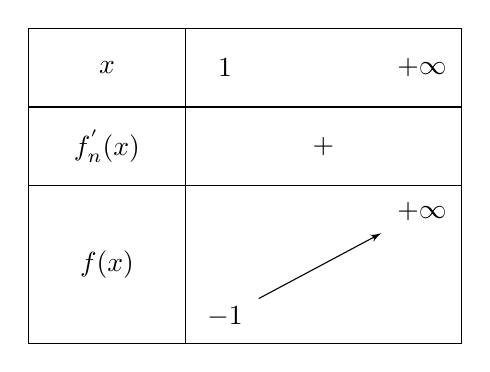
\begin{tikzpicture}
\tkzTabInit[lgt=2,espcl=2.5]
{$x $ / 1,$f_n^{'}(x)$ / 1, $f(x)$/2 }{$1$,$+\infty$}
\tkzTabLine{ , + ,   }
\tkzTabVar{-/$-1$,+/$+\infty$}
\end{tikzpicture}
\end{center}
La fonction $f_n$ est continue et strictement croissante sur $I$ (fonction polynômiale), $\dis \lim_{x \rightarrow 1} f_n(x)=-1$, $\dis \lim_{ x \rightarrow + \infty} f_n(x)= + \infty$ et $0 \in ]-1, + \infty [$. D'après le théorème de bijection, il existe un unique réel $x_n \in ]1, + \infty[$ tel que $f_n(x_n)=0.$
\item Pour tout réel $x \geq 1$, $f_{n+1}(x) = x^{n+1}-x-1$. Ainsi, $f_{n+1}(x_n)= x_n^{n+1}-x_n-1$. Or par définition , $f_n(x_n) = x_n^{n}-x_n-1 = 0$ ce qui est équivalent à $x_n^n = x_n+1$. Alors
\[ \begin{array}{ccl}
f_{n+1}(x_n) & = & x_n^{n+1}-x_n-1 \\
& = & x_n^n \times x_n - x_n - 1 \\
& = & (x_n+1) x_n -x_n -1 \\
& = & x_n^2 +x_n -x_n -1  \\
& = & x_n^2 - 1 \\
\end{array} \]
Or $x_n>1$ donc $x_n^2 > 1^2=1$ (par stricte croissance de la fonction carré sur $\mathbb{R}_+$) et ainsi $f_{n+1}(x_n)>0$.  On a donc $0=f_{n+1}(x_{n+1}) < f_{n+1}(x_n)$ et par stricte croissance de $f_{n+1}$ sur $I$ ($x_n$ et $x_{n+1}$ appartiennent à cet intervalle) on a $x_{n+1} < x_n$. Ainsi, $(x_n)_{n \geq 2}$ et strictement décroissante.
\item On sait que pour tout entier $n \geq 2$, $x_n >1$ la suite est donc minorée par $1$ (et décroissante d'après la question précédente). D'après le théorème de limite monotone, la suite est donc convergente vers un réel $\ell \geq 1$ (par passage à la limite avec les inégalités). 
\noindent Supposons par l'absurde que la suite $(x_n)_{n \geq 2}$ ne converge pas vers $1$. Elle converge donc vers un réel $\ell$ strictement plus grand que $1$ d'après la question précédente. Or on sait que pour tout $n \geq 2$, $f_n(x_n)=0$ ce qui est équivalent $x_n^n = x_n + 1$. On a $\dis \lim_{n \rightarrow + \infty} x_n + 1 = \ell + 1$. On remarque de plus que $\ln(x_n^n) = n \ln(x_n)$ ($x_n>0$ pour tout $n \geq 2$, on peut donc bien appliquer la fonction $\ln$). Or $\dis \lim_{n \rightarrow + \infty} \ln(x_n) = \ln(\ell)$ car $\ell >0$ et par composition de limites. De plus, $\ell>1$ donc $\ln(\ell) >0$ et ainsi $\dis \lim_{n \rightarrow + \infty} n \ln(x_n) = + \infty$ par produit de limites. Par composition avec la fonction exponentielle, on a alors 
\[ \lim_{n \rightarrow + \infty} x_n^n = \lim_{n \rightarrow + \infty} e^{n \ln(x_n)} = + \infty \]
Ceci est absurde car 
$$\dis \lim_{n \rightarrow + \infty} x_n^n = \lim_{n \rightarrow + \infty} x_n + 1 = \ell + 1 \in \mathbb{R}$$
Ainsi, par l'absurde, on a montré que $(x_n)_{n \geq 2}$ converge vers $1$.
\item Posons pour tout entier $n \geq 2$, 
$$ u_n = x_n -1$$
D'après la question précédente, $(u_n)_{n \geq 2}$ converge vers $0$.  On sait que pour tout entier $n \geq 2$,
$$ x_n^n = x_n + 1 >0$$
donc :
$$ (u_n+1)^n = u_n +2 $$
On sait que $x_n>1$ donc $u_n>0$ et :
$$ n \ln(u_n + 1) = \ln(u_n+2)$$
On sait que $\|n(u_n+1) \underset{+ \infty}{\sim} u_n$ donc :
$$ n \ln(u_n + 1) \underset{+ \infty}{\sim} nu_n$$
Par continuité du logarithme en $2$, on sait que :
$$ \lim_{n \rightarrow + \infty} \ln(u_n+2) = \ln(2)$$
donc :
$$ \lim_{n \rightarrow + \infty} n u_n = \ln(2)$$
et donc :
$$ u_n \underset{+ \infty}{\sim} \dfrac{\ln(2)}{n}$$
\end{enumerate}




\begin{Exa} \begin{enumerate}
\item Montrer que pour tout $n \geq 3$, $e^x=nx$ admet deux solutions $x_n$ et $y_n$ tels que $0 \leq x_n <y_n$.
\item Étudier la monotonie des suites $(x_n)$ et $(y_n)$ et en déduire qu'elles admettent une limite à déterminer.
\item Montrer que $x_n \underset{+ \infty}{\sim} \dfrac{1}{n}$, trouver un équivalent de $x_n - \dfrac{1}{n}$ quand $n$ tend vers $+ \infty$ et donner un développement asymptotique de $x_n$ à deux termes.
\item Soit $\varepsilon >0$. Montrer qu'à partir d'un certain rang, $y_n \leq (1+ \varepsilon) \ln(n)$. En déduire un équivalent de $y_n$ quand $n$ tend vers $+ \infty$.
\end{enumerate}
\end{Exa}

\corr \begin{enumerate}
\item Soit $n \geq 3$. On pose pour tout $x \geq 0$, $f_n(x)=e^x-nx$. La fonction $f_n$ est dérivable et pour tout $x \in \mathbb{R}_+$,
$$ f_n'(x)=e^x-n$$
La fonction $f_n$ est strictement décroissante sur $[0, \ln(n)]$ et est strictement croissante sur $[\ln(n), + \infty[$. On a de plus :
$$ f_n(0)=1, \; f_n(\ln(n))=n(1- \ln(n))<0 \hbox{ et } \lim_{x \rightarrow + \infty} f_n(x) = + \infty$$
par théorème des croissances comparées. Par double application du théorème des valeurs intermédiaires (la fonction $f_n$ étant continue sur $\mathbb{R}_+$), on en déduit qu'il existe deux uniques réels positifs $x_n$ et $y_n$ tels que $0 \leq x_n < \ln(n) < y_n$.
\item Soit $n \geq 3$.
\begin{itemize}
\item On sait que $f_{n+1}(x_{n+1})=0$, $f_{n+1}$ est décroissante sur $[0, \ln(n+1)]$, $x_n \in [0, \ln(n+1)]$ car $x_n \in [0, \ln(n)]$ et 
$$ f_{n+1}(x_n) = e^{x_n} - (n+1)x_n = e^{x_n} - nx_n - x_n = f_n(x_n)- x_n = -x_n \leq 0$$
donc $x_n \geq x_{n+1}$.
\item On sait que $f_{n}(y_{n})=0$, $f_{n}$ est croissante sur $[\ln(n), + \infty[$, $y_{n+1} \geq \ln(n)$ car $y_{n+1} \geq \ln(n+1)$ et 
$$ f_{n}(y_{n+1}) = e^{y_{n+1}} - ny_{n+1} = e^{y_{n+1}}-(n+1)y_{n+1} + y_{n+1} = f_{n+1}(y_{n+1})+y_{n+1}= y_{n+1} \geq 0$$
donc $y_{n+1} \geq y_n$.
\end{itemize}
On en déduit que $(x_n)$ est décroissante et que $(y_n)$ est croissante. On sait que pour tout $n \geq 3$,
$$ y_n \geq \ln(n)$$
donc par comparaison, on en déduit que $(y_n)$ diverge vers $+ \infty$. 

\medskip

\noindent La suite $(x_n)$ est décroissante et minorée par $0$ donc elle converge vers un réel $\ell \geq 0$. Supposons par l'absurde que $\ell>0$. On sait que pour tout $n \geq 0$, $f_n(x_n)=0$ donc :
$$e^{x_n} = nx_n$$
Par continuité de l'exponentielle en $\ell$, on sait que :
$$ \lim_{n \rightarrow + \infty} e^{x_n} = e^{\ell}$$
et on a :
$$ \lim_{n \rightarrow + \infty} nx_n = + \infty$$
ce qui est absurde. Ainsi, $(x_n)$ converge vers $0$.
\item Pour tout $n \geq 3$, $f_n(x_n)=0$ donc $e^{x_n} = nx_n$. Sachant que $(x_n)$ converge vers $0$, on a par continuité de l'exponentielle en $0$ :
$$ \lim_{n \rightarrow + \infty} e^{x_n} = 1$$
donc :
$$ \lim_{n \rightarrow + \infty} n x_n = 1$$
et ainsi,
$$x_n \underset{+ \infty}{\sim} \dfrac{1}{n}$$
Posons pour tout $n \geq 3$,
$$ u_n = x_n - \dfrac{1}{n}$$
et donc :
$$ nx_n =1+n u_n $$
On sait que :
$$ \lim_{n \rightarrow + \infty} n x_n = 1$$
donc 
$$ \lim_{n \rightarrow + \infty} n u_n = 0$$
Pour tout $n \geq 3$, $x_n >0$ et on a :
$$ \ln(nx_n) = \ln(1+n u_n) \underset{+ \infty}{\sim} n u_n$$
Or on sait que $e^{x_n}=nx_n$ donc $x_n = \ln(nx_n)$ ce qui implique que :
$$ x_n \underset{+ \infty}{\sim} n u_n $$
et donc par transitivité :
$$ n u_n \underset{+ \infty}{\sim}  \dfrac{1}{n}$$
et ainsi :
$$ u_n \underset{+ \infty}{\sim}  \dfrac{1}{n^2}$$
ce qui implique que :
$$ u_n \underset{+ \infty}{=} \dfrac{1}{n^2} + o \left( \dfrac{1}{n^2} \right)$$
et finalement :
$$ x_n  \underset{+ \infty}{=} \dfrac{1}{n} + \dfrac{1}{n^2} + o \left( \dfrac{1}{n^2} \right)$$
\item Soit $\varepsilon >0$. On sait que $(1+ \varepsilon) \ln(n) \geq \ln(n)$ et $y_n \geq \ln(n)$ donc par croissance de $f_n$ sur $[\ln(n), + \infty[$, on a :
\begin{align*}
y_n \leq (1+ \varepsilon) \ln(n)&  \Longleftrightarrow f_n(y_n) \leq f_n((1+ \varepsilon) \ln(n)) \\
 & \Longleftrightarrow 0 \leq e^{(1+ \varepsilon) \ln(n)} - n (1+ \varepsilon) \ln(n) \\
 & \Longleftrightarrow 0 \leq n^{1+ \varepsilon} - n(1+ \varepsilon) \ln(n) 
 \end{align*}
Cette dernière inégalité est vraie à partir d'un certain rang car par théorème des croissances comparées :
$$ \lim_{n \rightarrow + \infty}  n^{1+ \varepsilon} - n(1+ \varepsilon) \ln(n)  = + \infty$$
Finalement pour tout $\varepsilon>0$, il existe un rang $N \geq 3$ tel que pour tout $n \geq N$,
$$ \ln(n) \leq y_n \leq (1+ \varepsilon) \ln(n)$$
ou encore 
$$ 1 \leq \dfrac{y_n}{\ln(n)} \leq 1+ \varepsilon$$
puis 
$$ 0 \leq \dfrac{y_n}{\ln(n)} - 1 \leq \varepsilon$$
et donc :
$$ \left\vert \dfrac{y_n}{\ln(n)} - 1 \right\vert \leq \varepsilon$$
Par définition de convergence, on en déduit que :
$$ \lim_{n \rightarrow + \infty} \dfrac{y_n}{\ln(n)} = 1$$
et ainsi :
$$ y_n \underset{+ \infty}{\sim} \ln(n)$$

\end{enumerate}




\begin{Exa} D\'{e}terminer le signe, au voisinage de l'infini, de 
$$u_{n}=\text{sh}\left( \dfrac{1}{n}\right) -\tan \left( \dfrac{1}{n}\right)$$
\end{Exa}

\corr On utilise les développements limités de $\sh$ et $\tan$ en $0$ sachant que $\dfrac{1}{n}$ tend vers $0$ quand $n$ tend vers $+ \infty$ : 
$$\textrm{sh} \left(\dfrac{1}{n} \right) \underset{+ \infty}{=} \dfrac{1}{n} + \dfrac{1}{{6n^3 }} + o\left( {\dfrac{1}{{n^3 }}} \right) \; \hbox{ et } \tan \left(\dfrac{1}{n}\right) \underset{+ \infty}{=} \dfrac{1}{n} + \dfrac{1}{{3n^3 }} + o\left( {\dfrac{1}{{n^3 }}} \right)$$
Ainsi :
$$u_n  \underset{+ \infty}{\sim } - \dfrac{1}{{6n^3 }}$$
D'après la première question, on en déduit qu'à partir d'un certain rang, $u_n$ et $ - \dfrac{1}{{6n^3 }}$ sont de même signe donc $u_n$ est négatif.

\end{document}